% This LaTeX document needs to be compiled with XeLaTeX.
\documentclass[10pt]{article}
\usepackage[utf8]{inputenc}
\usepackage{amsmath}
\usepackage{amsfonts}
\usepackage{amssymb}
\usepackage[version=4]{mhchem}
\usepackage{stmaryrd}
\usepackage{graphicx}
\usepackage[export]{adjustbox}
\graphicspath{ {./images/} }
\usepackage[fallback]{xeCJK}
\usepackage{polyglossia}
\usepackage{fontspec}
\setCJKmainfont{Noto Serif CJK JP}

\setmainlanguage{polish}
\setmainfont{CMU Serif}

\title{LIGA MATEMATYCZNA \\
 FINAモ \\
 30 marca 2011 \\
 SZKOŁA PODSTAWOWA }

\author{}
\date{}


\begin{document}
\maketitle
\section*{ZADANIE 1.}
Trapez o obwodzie 72 cm podzielono wysokościami na dwa trójkąty i prostokąt. Suma obwodów tych trzech figur jest równa 142 cm . Oblicz wysokość tego trapezu.

\section*{ZADANIE 2.}
\(1=1^{2}-0^{2}\)\\
\(3=2^{2}-1^{2}\)\\
\(5=3^{2}-2^{2}\)\\
Napisz trzy kolejne wiersze. Przedstaw liczbę 2011 w postaci różnicy kwadratów dwóch liczb naturalnych.

\section*{ZADANIE 3.}
Skrzynia, kufry i pudełka mają zamki. W skrzyni jest sześć kufrów, w każdym kufrze są po trzy pudełka, a w każdym pudełku po trzy złote monety. Jaka jest najmniejsza liczba zamków, które trzeba otworzyć, aby wyjąć 22 złote monety?

\section*{ZADANIE 4.}
W pewnej klasie jest 30 uczniów. Wśród nich pięciu ma brata i siostrę, a siedmiu nie ma brata ani siostry. Ilu uczniów tej klasy ma brata, jeżeli wiadomo, że trzynastu ma siostrę?

\section*{ZADANIE 5.}
W dane kółka wpisz liczby tak, aby suma liczb w każdych trzech kolejnych kółkach była równa 15.\\
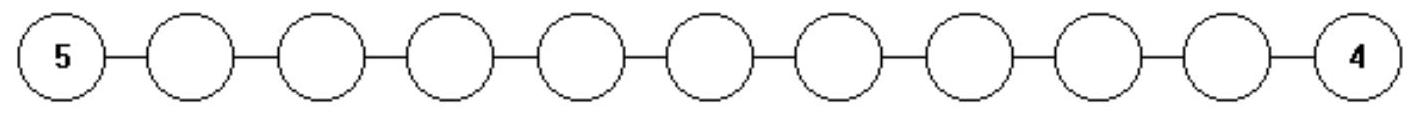
\includegraphics[max width=\textwidth, center]{2024_11_21_2300f3f933ebda9c3480g-1}


\end{document}